\documentclass[12pt]{article}

\usepackage[margin=1.5cm]{geometry}        % For setting margins
\usepackage[spanish,es-tabla]{babel}
\selectlanguage{spanish}
\usepackage{amsmath}                % For Math
\usepackage{fancyhdr}                % For fancy header/footer
\usepackage{graphicx}                % For including figure/image
\usepackage{cancel}                    % To use the slash to cancel out stuff in working out equations
\usepackage{amsfonts}
\usepackage{color}
\usepackage{bbm}
\usepackage{float}
\usepackage{subcaption}
\usepackage{lipsum}
\usepackage{listings}
\usepackage{algorithm,algpseudocode}
\usepackage{hyperref}
\usepackage{amssymb}
\usepackage{tikz}
\usepackage{booktabs}
\usetikzlibrary{arrows, positioning}
\captionsetup{compatibility=false}

%%%%%%%%%%%%%%%%%%%%%%
% Set up fancy header/footer
\pagestyle{fancy}
\fancyhead[LO,L]{Alejandro Uribe}
\fancyhead[CO,C]{}
\fancyhead[RO,R]{Aprendizaje Reforzado - Guía 2: Procesos de Decisión Markovianos}
\fancyfoot[LO,L]{}
\fancyfoot[CO,C]{\thepage}
%\fancyfoot[RO,R]{\today}
\renewcommand{\headrulewidth}{0.4pt}
\renewcommand{\footrulewidth}{0.4pt}

\newlength\tindent
\setlength{\tindent}{\parindent}
\setlength{\parindent}{0pt}
\renewcommand{\indent}{\hspace*{\tindent}}
\DeclareMathOperator*{\argmax}{argmax}
\floatname{algorithm}{Algoritmo}

\decimalpoint
\bibliographystyle{ieeetr}
%%%%%%%%%%%%%%%%%%%%%%

\begin{document}
    \indent\underline{\textbf{Ejercicio 1}}\\
\textcolor{green}{[Programación]} Para el proceso de Markov de recompensas (MRP) de la figura~\ref{fig:grafo_ej_1}, calcular los valores de los estados de forma iterativa con los siguientes algoritmos y compare sus convergencias.
Considere factor de descuento $\gamma < 0.9$.\\

\begin{figure}[H]
    \centering
    \begin{tikzpicture}[->, >=stealth', auto, semithick, node distance=2cm]
        % Nodes
        \node[circle, draw] (s1) {$s_1$};
        \node[circle, draw, right=of s1] (s2) {$s_2$};
        % Arrows
        \path (s1) edge[bend left=60] node {R=1} (s2)
              (s2) edge[bend left=60] node[align=center] {R=2 \\ $p(s_2 \mid s_1) = 1$ \\ $p(s_1 \mid s_2) = 1$} (s1);
    \end{tikzpicture}
    \caption{Grafo de transición de estados}\label{fig:grafo_ej_1}
\end{figure}


\begin{itemize}
    \item Actualizar todos los valores a la vez por iteración: $v_{k+1} = r + \gamma P v_k$, con $v_k\, r$ siendo los vectores de valores y recompensas, respectivamente; y $P$ la matriz de probabilidades de transición.
    \item Actualizar los valores de un estado por vez \textit{(in place)}: $v_{k+1}(s') = r(s') + \gamma v_k(s)$, con $v_k(s)$ y $r(s')$ siendo los valores y recompensas correspondientes a los estados $s$ y $s'$, respectivamente.
\end{itemize}

\indent\underline{\textbf{Solución}}\\
La implementación de los algoritmos se realizó en Python, que se puede encontrar en el repositorio de \href{https://github.com/MasterUBA-DM-KD/Aprendizaje_Reforzado/blob/5ae50da937b14f0a11c416e40019a4b5661dd51b/docs/guia/3/notebooks/utils.py}{GitHub}.

Sea, $P$ la matriz de probabilidades de transición:

\[
  P = \begin{bmatrix} 0 & 1 \\ 1 & 0 \end{bmatrix}
\]

Sea $r$ el vector de recompensas:

\[
  r = \begin{bmatrix} 1 \\ 2 \end{bmatrix}
\]

A continuación los resultados de los valores de los estados para $\gamma \in [0, 0.9)$ usando los métodos \textit{iterativo} e \textit{in place}.

\paragraph{Método \textit{iterativo}} Se calculó el vector de valor $v_{k+1}$ usando el cálculo iterativo con la librería \texttt{numpy} de Python\footnotemark.
La figura~\ref{fig:iter_gamma_vk} muestra los valores de $v_{k+1}$ y la figura~\ref{fig:iter_gamma_iter} muestra el número de iteraciones necesarias para converger, ambas para $\gamma \in [0, 0.9)$.

\footnotetext{Se una tolerancia de $10^{-6}$ y un máximo de $1000$ iteraciones.}

La figura~\ref{fig:iter_gamma} muestra los resultados para el método \textit{iterativo}.

\begin{figure}[H]
    \centering
    \begin{subfigure}[H]{0.45\textwidth}
        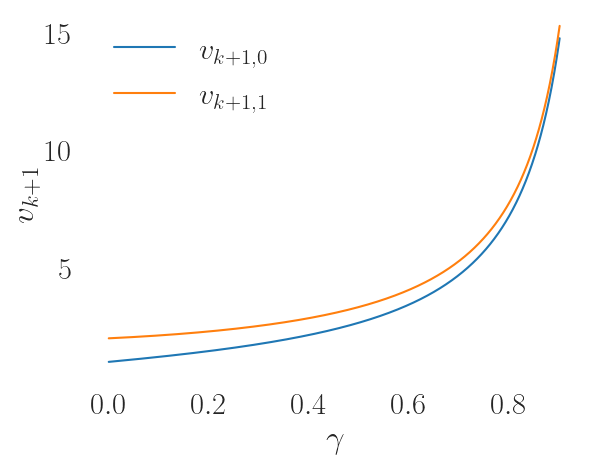
\includegraphics[width=\textwidth]{../img/gamma_v_k}
        \caption{Vector de valores}
        \label{fig:iter_gamma_vk}
    \end{subfigure}
    \begin{subfigure}[H]{0.45\textwidth}
        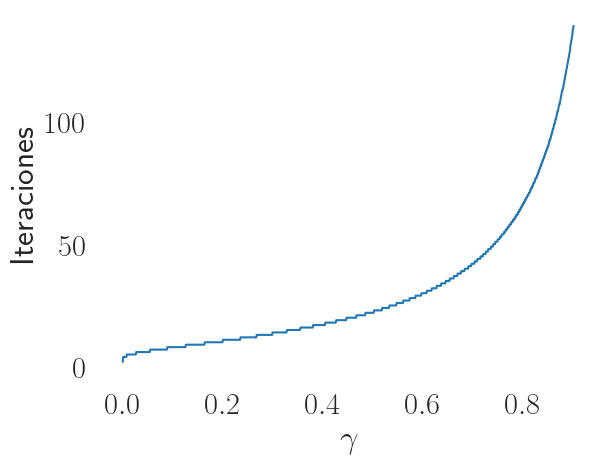
\includegraphics[width=\textwidth]{../img/gamma_iters}
        \caption{Número de iteraciones para converger}
        \label{fig:iter_gamma_iter}
    \end{subfigure}
    \caption{Resultados del método \textit{iterativo}}\label{fig:iter_gamma}
\end{figure}

\paragraph{Método \textit{in place}} Se calculó el vector de valor $v_{k+1}$ usando el cálculo iterativo con la librería \texttt{numpy} de Python\footnotemark.
La figura~\ref{fig:inplace_gamma_vk} muestra los valores de $v_{k+1}$ y la figura~\ref{fig:inplace_gamma_iter} muestra el número de iteraciones necesarias para converger, ambas para $\gamma \in [0, 0.9)$.

\footnotetext{Se fijó una tolerancia de $10^{-6}$ y un máximo de $1000$ iteraciones.}

La figura~\ref{fig:inplace_gamma} muestra los resultados para el método \textit{in place}.

\begin{figure}[H]
    \centering
    \begin{subfigure}[H]{0.45\textwidth}
        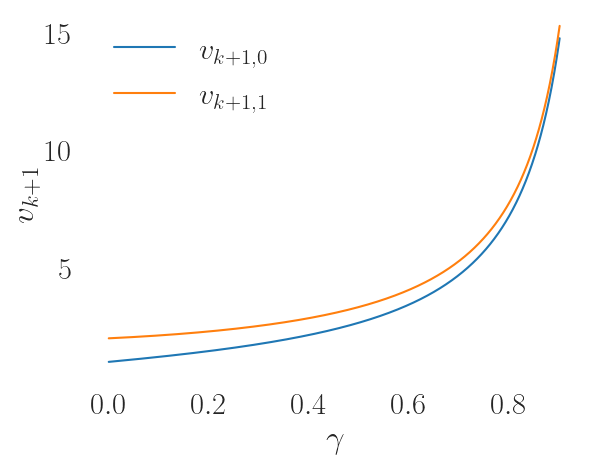
\includegraphics[width=\textwidth]{../img/gamma_v_k}
        \caption{Vector de valores}
        \label{fig:inplace_gamma_vk}
    \end{subfigure}
    \begin{subfigure}[H]{0.45\textwidth}
        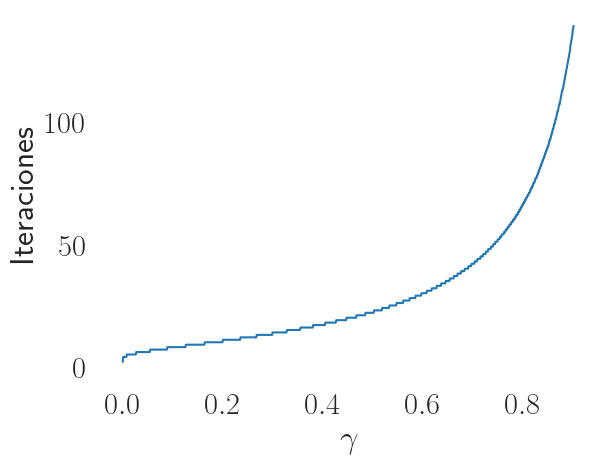
\includegraphics[width=\textwidth]{../img/gamma_iters}
        \caption{Número de iteraciones para converger}
        \label{fig:inplace_gamma_iter}
    \end{subfigure}
    \caption{Resultados del método \textit{inplace}}\label{fig:inplace_gamma}
\end{figure}

\indent\underline{\textbf{Conclusiones}}\\
No existe una diferencia significativa entre los métodos \textit{iterativo} e \textit{in place} para valores de $\gamma \in [0, 0.9)$.
A continuación se presentan las conclusiones de los resultados obtenidos.

\paragraph{Vector de valores $v_{k+1}$}
Las figuras~\ref{fig:iter_gamma_vk} y~\ref{fig:inplace_gamma_vk} muestran los valores de $v_{k+1}$ para $\gamma \in [0, 0.9)$ para los métodos \textit{iterativo} e \textit{in place}, respectivamente.
De las figuras se concluye,

\begin{itemize}
    \item Ambos métodos mostraron una rápida convergencia cuando $\gamma \approx 0$, dando como resultado $v_{k+1} = r = \begin{bmatrix} 1 \\ 2 \end{bmatrix}$.
    \item Los valores de $v_{k+1}$ aumentan de forma exponencial a medida que $\gamma$ aumenta.
    \item Conforme $\gamma \rightarrow 0.9$, los métodos convergen a los valores teóricos $v = \begin{bmatrix} 14.74 \\ 15.26 \end{bmatrix}$.
\end{itemize}

\paragraph{Iteraciones}
Las figuras~\ref{fig:iter_gamma_iter} y~\ref{fig:inplace_gamma_iter} muestran el número de iteraciones necesarias para converger para $\gamma \in [0, 0.9)$ para los métodos \textit{iterativo} e \textit{in place}, respectivamente.
De las figuras se concluye,

\begin{itemize}
    \item Las iteraciones necesarias para converger aumentan de forma exponencial a medida que $\gamma$ aumenta.
    \item Conforme $\gamma \rightarrow 0.9$, se requieren más iteraciones para converger, lo que se traduce en un mayor tiempo de cómputo.
\end{itemize}

\paragraph{Implementación}En cuanto a la implementación de ambos métodos, la diferencia entre el método \textit{iterativo} e \textit{in place} radica en que el segundo no requiere de una matriz de transición $P$.
Desde una perspectiva computacional el método \textit{in place} es más eficiente, ya que no requiere de una matriz de transición.
También es útil en escenarios en los que la matriz de transición no es conocida, como en el caso de un agente que interactúa con un entorno desconocido.

\line(1,0){\textwidth}

    \indent\underline{\textbf{Ejercicio 2}}\\
Demostrar que la política $\varepsilon \text{ - \textit{Greedy}}$, definida de la siguiente manera

\begin{equation}
\pi(a|s) = \left\{
\begin{array}{lcc}
    1 - \varepsilon + \frac{\varepsilon}{|A(s)|} & si  & a = a^{\ast} \\ \\
     \frac{\varepsilon}{|A(s)|} &  si & a \neq a^{\ast}
\end{array}
   \right.\label{eq:equation}
\end{equation}

es una distribución de probabilidad válida, donde $|A(s)|$ es el número de acciones para el estado $s, \ \varepsilon < 1$ es un número positivo pequeño, y $a^{\ast}$ es la acción óptima (decisión greedy) para el estado $s$.
¿Hay que pedir alguna condición sobre $\varepsilon$?

\indent\underline{\textbf{Solución}}\\

\line(1,0){\textwidth}


    \indent\underline{\textbf{Ejercicio 3}}\\
En el Ejemplo 4.1 (\textit{GridWorld}, Sutton\&Barto, 2018)~\cite{Sutton2018}, suponga que se agrega un nuevo estado $15$ debajo del estado $13$ y sus acciones: \textit{left, up, right} y \textit{down}, lleva al agente a los estados $12$, $13$, $14$ y $15$, respectivamente.

\begin{itemize}
    \item Considere que las transiciones desde los estados originales no se cambian.
    ¿Cuánto vale $v_{\pi}(15)$ para la política $\pi$ aleatoria y equiprobable?
    Utilice $v(12) = -22$, $v(13) = -20$, $v(14) = -14$ (figura~\ref{fig:gridworld}).
\end{itemize}

Justifique su respuesta.

\indent\underline{\textbf{Solución}}\\
Sea,\\
$p(s',r|s,a) = 0.25, \ \forall s \in S, \forall a \in A$\\

La función de valor de estado $v_{\pi}(s)$ para la política $\pi$ es:

\[
    v_{pi} = \sum_{a} \pi(a|s) \sum_{s',r} p(s',r|s,a) \left[ r + \gamma v_{\pi}(s') \right]
\]

Para calcular $v_{\pi}(15)$,

\begin{align*}
    v_{\pi}(15) &= \sum_{a} \pi(a|15) \sum_{s',r} p(s',r|15,a) \left[ r + \gamma v_{\pi}(s') \right] \\
    &= 0.25 \left[ r + \gamma v_{\pi}(s') \right] \\
    &= 0.25 \left[\left(-1 -20 \right) + \left(-1 -22 \right) + \left(-1 -14 \right) + \left(-1 + v_{\pi}(15) \right) \right] \\
    &= 0.25 \left[ -21 -23 -15 -1 + v_{\pi}(15) \right] \\
    &= 0.25 \left[ -60 + v_{\pi}(15) \right] \\
    &= -15 + 0.25 \cdot v_{\pi}(15)
\end{align*}

Al considerar que las transiciones desde los estados originales no se cambian, es posible la transición del estado $13$ al $15$.
Pasar al estado $15$ tiene un valor igual al del estado $13$.
Por lo tanto,

\begin{align*}
    v_{\pi}(15) &= v_{\pi}(13) \\
    &= -20
\end{align*}

Al reemplazar $v_{\pi}(15)$ en la ecuación anterior, se obtiene:

\begin{align*}
    v_{\pi}(15) &= -15 + 0.25 \cdot v_{\pi}(15) \\
    &= -15 + 0.25 \cdot (-20) \\
    &= -15 - 5 \\
    &= -20
\end{align*}

\line(1,0){\textwidth}


    \indent\underline{\textbf{Ejercicio 4}}\\
En el Ejemplo 4.3 (\textit{Gambler’s problem, Sutton\&Barto, 2018})~\cite{Sutton2018}, la política óptima tiene una forma particular (ver figura~\ref{fig:gamblers_problem}) con máximo en $50$.
Es decir, cuando el jugador tiene $\$50$, le conviene apostarlo todo; sin embargo, cuando tiene $\$51$, le conviene apostar $\$1$.
¿Por qué sucede esto?

\begin{figure}[H]
    \centering
    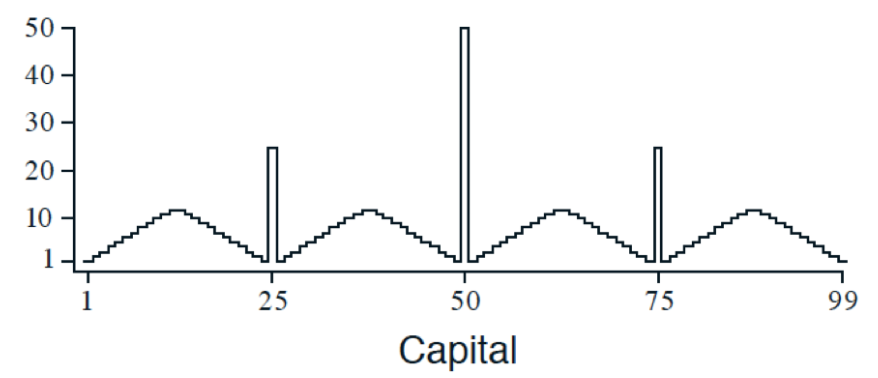
\includegraphics[width=0.5\textwidth]{../img/gamblers_problem}
    \caption{Ejemplo 4.3~\cite{Sutton2018}}
    \label{fig:gamblers_problem}
\end{figure}

\indent\underline{\textbf{Solución}}\\
El ejemplo 4.3 (\textit{Gambler’s problem, Sutton\&Barto, 2018})~\cite{Sutton2018} se plantea como un MDP finito, sin descuento, episódico y con un conjunto de estados $s \in \left\{0, 1, \ldots, 99\right\}$ y un conjunto de acciones $a \in \left\{0, 1, \ldots, \min(s, 100-s)\right\}$.

Por otro lado, la política final encontrada es tal que $p_h=0.4$, es decir, la probabilidad de que la moneda salga cara es $0.4$.

Por lo tanto, cuando la moneda está cargada y al jugador le conviene minimizar el número de apuestas realizadas porque en el largo plazo, el jugador perderá dinero.
Por lo tanto, el jugador tiene una \textit{ventaja}\footnotemark y le conviene apostar todo cuando tiene $\$50$, ya que a la izquierda y derecha de este valor las apuestas llevarán al jugador de vuelta a $\$50$.
Por lo que si tiene $\$51$ le conviene apostar $\$1$ sabiendo que si pierde, volverá a $\$50$.
\footnotetext{La ventaja se refiere a que si el jugador apuesta los $\$50$ tendrá el $40\%$ de probabilidad de ganar.}

\line(1,0){\textwidth}


    \indent\underline{\textbf{Ejercicio 5}}\\
\textcolor{green}{[Programación]} Implemente el Algoritmo de Iteración de Valores para el el Ejemplo 4.3 (\textit{Gambler’s problem, Sutton\&Barto, 2018})~\cite{Sutton2018} para los siguientes casos:

\begin{itemize}
    \item $p_h = 0.25$.
    \item $p_h = 0.55$.
\end{itemize}

Compare los resultados y saque conclusiones.

\indent\underline{\textbf{Solución}}\\
La implementación de los algoritmos se realizó en Python, que se puede encontrar en el repositorio de \href{https://github.com/MasterUBA-DM-KD/Aprendizaje_Reforzado/blob/5ae50da937b14f0a11c416e40019a4b5661dd51b/docs/guia/3/notebooks/utils.py}{GitHub}.

Sea,\\
$N=100$: capital máximo\\
$S=\left\{0, 1, \ldots, 100\right\}$: conjunto de estados\\
$A=\left\{0, 1, \ldots, \min(s, 100-s)\right\}$: conjunto de acciones\\

El Algoritmo de Iteración de Valores para el Ejemplo 4.3 (\textit{Gambler’s problem, Sutton\&Barto, 2018})~\cite{Sutton2018} se implementó en Python\footnotemark.
A continuación, los resultados de la implementación, $p_h = 0.25$, se muestran en las figuras~\ref{fig:ph_025_sweeps} y~\ref{fig:ph_025_policy}.

\footnotetext{Se fijó una tolerancia de $10^{-3}$ para la convergencia.}

\begin{figure}[H]
    \centering
    \begin{subfigure}[H]{0.45\textwidth}
        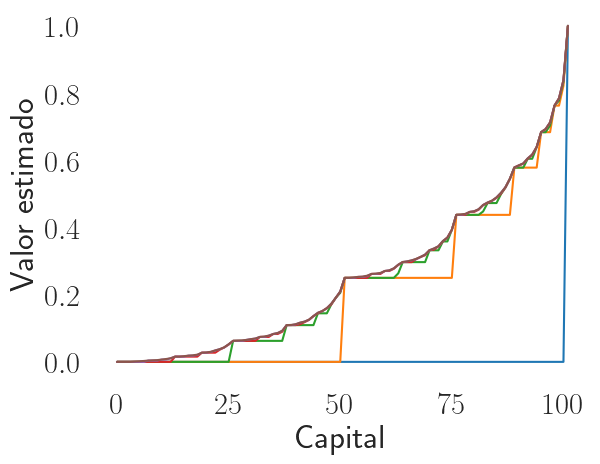
\includegraphics[width=\textwidth]{../img/sweeps_0.25}
        \caption{$sweeps \in [0, N]$}
        \label{fig:ph_025_sweeps}
    \end{subfigure}
    \begin{subfigure}[H]{0.45\textwidth}
        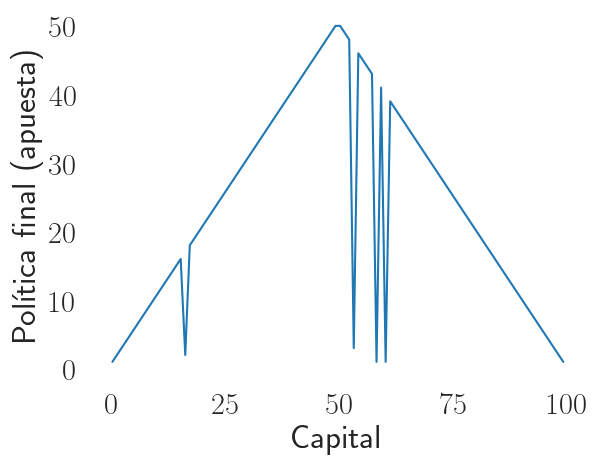
\includegraphics[width=\textwidth]{../img/policy_0.25}
        \caption{Política final}
        \label{fig:ph_025_policy}
    \end{subfigure}
    \caption{$ph=0.25$}
    \label{fig:ph_025_gamblers_problem}
\end{figure}

A continuación, los resultados de la implementación, $p_h = 0.55$, se muestran en las figuras~\ref{fig:ph_055_sweeps} y~\ref{fig:ph_055_policy}.

\begin{figure}[H]
    \centering
    \begin{subfigure}[H]{0.45\textwidth}
        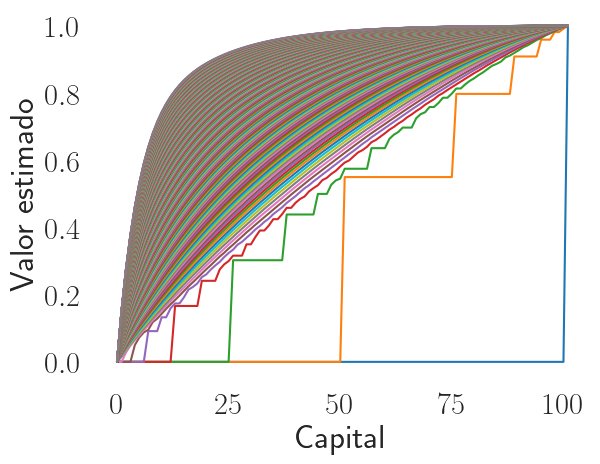
\includegraphics[width=\textwidth]{../img/sweeps_0.55}
        \caption{$sweeps \in [0, N]$}
        \label{fig:ph_055_sweeps}
    \end{subfigure}
    \begin{subfigure}[H]{0.45\textwidth}
        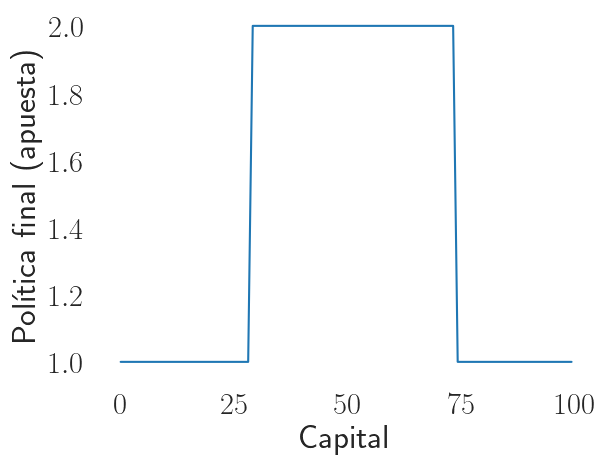
\includegraphics[width=\textwidth]{../img/policy_0.55}
        \caption{Política final}
        \label{fig:ph_055_policy}
    \end{subfigure}
    \caption{$ph=0.55$}
    \label{fig:ph_055_gamblers_problem}
\end{figure}

\indent\underline{\textbf{Conclusiones}}
\paragraph{Convergencia} En las figuras~\ref{fig:ph_025_sweeps} y~\ref{fig:ph_055_sweeps} se muestra que a medida que se aumentan las iteraciones (sweeps), los valores de vada estado convergen a un valor estable.

\paragraph{Política final} Se encuentra influenciada por el valor de $p_h$.
Cuando la probabilidad de ganar es baja la política óptima es apostar poco, especialmente cuando el capital es bajo, hecho que se deba al alto riesgo de perder el capital.
Además, para este caso la política final tiene forma de \textit{V} invertida como se muestra en la figura~\ref{fig:ph_025_policy}.

Por otro lado, cuando la probabilidad de ganar es alta, la política óptima es apostar más, especialmente cuando el capital es intermedio, hecho que se debe a la alta probabilidad de ganar y la posibilidad de maximizar la ganancia.
Además, para este caso la política final tiene forma de \textit{V} achatada, como se muestra en la figura~\ref{fig:ph_055_policy}.

En ambos casos:
\begin{itemize}
    \item Se apuesta poco si se tiene poco capital para evitar perderlo.
    \item Se apuesta más si se tiene un capital intermedio, aprovechando la oportunidad de ganar.
    \item Se apuesta poco si se tiene mucho capital para asegurar ganancia.
\end{itemize}

Se hace la salvedad que en el caso de $p_h = 0.25$ la política final tiene un máximo en el que se encuentra poca estabilidad.

\line(1,0){\textwidth}


    \indent\underline{\textbf{Ejercicio 6}}\\
Demostrar la ecuación de \textit{Bellman} para MRPs con $N$ estados

\[
    v = r + \gamma Pv,
\]

donde $v \in \mathbb{R}^N$ es el vector de valores de estados, $r \in \mathbb{R}^N$ es el vector de recompensas medias partiendo de cada estado, $P \in \mathbb{R}^{N \times N} $ es la matriz de transiciones y $\gamma$ es el factor de descuento.

\indent\underline{\textbf{Solución}}\\
Sea,\\
$v \in \mathbb{R}^N$: Vector de valores de estados.\\
$r \in \mathbb{R}^N$: Vector de recompensas medias partiendo de cada estado.\\
$P \in \mathbb{R}^{N \times N}$: Matriz de transiciones.\\
$\gamma \in \left[0,1\right)$: Factor de descuento. \\
$i$: Índice del estado.

Partiendo de la ecuación de \textit{Bellman} para un estado $i$,

\[
    v_i = r_i + \gamma \sum_{j=1}^{N} P_{ij} v_j
\]

Es decir, el valor de un estado $i$ es la recompensa inmediata $r_i$ más el valor esperado de los estados siguientes ponderados por la probabilidad de transición desde $i$ a $j$, $P_{ij}$, siendo la matriz de transiciones, y descontados por el factor $\gamma$.
El primer término se puede expresar en forma matricial como,

\[
    r
\]

El segundo término es la suma ponderada de los valores de los estados siguientes.

\[
    \gamma \sum_{j=1}^{N} P_{ij} v_j
\]

Es decir, el factor de descuento $\gamma$ resta valor a los estados futuros~\cite{Sutton2018}.
Este término se puede expresar en forma matricial como,

\[
    \gamma Pv
\]

Al sumar ambos términos se obtiene la ecuación de \textit{Bellman} para MRPs con $N$ estados,

\[
    v = r + \gamma Pv
\]

\line(1,0){\textwidth}


    \indent\underline{\textbf{Ejercicio 7}}\\
\textcolor{green}{[Programación]} Resuelva la ecuación de Bellman para el MRP del Ejercicio 4 por los siguientes métodos para $\gamma \in \left\{0, 0.5, 0.9\right\}$:

\begin{enumerate}
    \item Iterando $v_{n+1} = r + \gamma P v_n$
    \item Usando algún método iterativo para resolver sistemas lineales, por ejemplo usando eliminación Gaussiana (vía \textit{numpy.linalg.solve()})
    \item Calculando la inversa de la matriz $I - \gamma P$
\end{enumerate}

\indent\underline{\textbf{Solución}}\\


Se tiene la matriz de transición $P$, mostrada en la Tabla~\ref{tab:p_matrix}.

\begin{table}[H]
    \centering
    \caption{Matriz de transición}
    \label{tab:p_matrix}
    \begin{tabular}{l|l|l|l|l|l|l|l}
        & FB  & C1                     & C2  & C3  & Pub & Pass & Sleep \\ \hline
        FB    & 0.9 & 0.1                    & 0   & 0   & 0   & 0    & 0     \\ \hline
        C1    & 0.5 & \multicolumn{1}{c|}{0} & 0.5 & 0   & 0   & 0    & 0     \\ \hline
        C2    & 0   & \multicolumn{1}{c|}{0} & 0   & 0.8 & 0   & 0    & 0.2   \\ \hline
        C3    & 0   & \multicolumn{1}{c|}{0} & 0   & 0   & 0.4 & 0.6  & 0     \\ \hline
        Pub   & 0   & 0.2                    & 0.4 & 0.4 & 0   & 0    & 0     \\ \hline
        Pass  & 0   & 0                      & 0   & 0   & 0   & 0    & 1     \\ \hline
        Sleep & 0   & 0                      & 0   & 0   & 0   & 0    & 0
    \end{tabular}
\end{table}

El vector de recompensas $r$, se muestra en la Tabla~\ref{tab:r_vector}.

\begin{table}[H]
    \centering
    \caption{Vector de recompensas}
    \label{tab:r_vector}
    \begin{tabular}{l|l}
        & $r_i$ \\ \hline
        FB    & -1    \\ \hline
        C1    & -2    \\ \hline
        C2    & -2    \\ \hline
        C3    & -2    \\ \hline
        Pub   & 1     \\ \hline
        Pass  & 10    \\ \hline
        Sleep & 0
    \end{tabular}
\end{table}

\paragraph{Método 1: Iterando $v_{n+1} = r + \gamma P v_n$}
Se iteró el cálculo de $v_{n+1}$ hasta que la diferencia entre $v_{n+1}$ y $v_n$ sea menor a $10^{-6}$.
A continuación se muestran los valores de $v_{n+1}$ para $\gamma \in {0,0.5,0.9}$ en la Tabla~\ref{tab:v_iter}\footnotemark.

\footnotetext{El cálculo se hizo con Excel, la hoja de cálculo utilizada se encuentra disponible en el repositorio de \href{https://github.com/MasterUBA-DM-KD/Aprendizaje_Reforzado/blob/4993e3466d1afb2b2c57489c20714a0b8106d984/docs/guia/1/notebooks/armed_bandits.py}{GitHub}.}

\begin{table}[H]
    \centering
    \caption{Método iterativo - Valores de $v_{n+1}$ para $\gamma \in {0,0.5,0.9}$}
    \label{tab:v_iter}
    \begin{tabular}{l|l|l|l}
        & $\gamma=0$ & $\gamma=0.5$ & $\gamma=0.9$ \\ \hline
        FB    & -1.000    & -2.083         & -7.6438         \\ \hline
        C1    & -2.000    & -2.908         & -5.013         \\ \hline
        C2    & -2.000    & -1.550         & 0.943         \\ \hline
        C3    & -2.000    & 1.125         & 4.087         \\ \hline
        Pub   & 1.000     & 0.624          & 1.908          \\ \hline
        Pass  & 10.000    & 10.000           & 10.000           \\ \hline
        Sleep & 0.000     & 0.000            & 0.000
    \end{tabular}
\end{table}

\paragraph{Método 2: Usando eliminación Gaussiana}
Se realizó el cálculo de $v$ para $\gamma \in {0,0.5,0.9}$ usando eliminación Gaussiana, con ayuda de la función \textit{numpy.linalg.solve()}.
A continuación se muestran los valores de $v$ en la Tabla~\ref{tab:v_gauss}\footnotemark.

\footnotetext{El cálculo se hizo con NumPy, el código utilizado se encuentra disponible en el repositorio de \href{https://github.com/MasterUBA-DM-KD/Aprendizaje_Reforzado/blob/4993e3466d1afb2b2c57489c20714a0b8106d984/docs/guia/1/notebooks/armed_bandits.py}{GitHub}.}

\begin{table}[H]
    \centering
    \caption{Método de eliminación Gaussiana - Valores de $v$ para $\gamma \in {0,0.5,0.9}$}
    \label{tab:v_gauss}
    \begin{tabular}{l|l|l|l}
        & $\gamma=0$ & $\gamma=0.5$ & $\gamma=0.9$ \\ \hline
        FB    & -1.000    & -2.082         & -7.637         \\ \hline
        C1    & -2.000    & -2.908         & -5.013         \\ \hline
        C2    & -2.000    & -1.550         & 0.943         \\ \hline
        C3    & -2.000    & 1.125         & 4.087         \\ \hline
        Pub   & 1.000     & 0.624          & 1.908          \\ \hline
        Pass  & 10.000    & 10.000           & 10.000           \\ \hline
        Sleep & 0.000     & 0.000            & 0.000
    \end{tabular}
  \end{table}

\paragraph{Método 3: Calculando la inversa de la matriz $I - \gamma P$}
Para calcular la inversa de la matriz $I - \gamma P$, se utilizó la función \textit{numpy.linalg.inv()}.
A continuación se muestran los valores de $v$ en la Tabla~\ref{tab:v_inv}\footnotemark.

\footnotetext{El cálculo se hizo con NumPy, el código utilizado se encuentra disponible en el repositorio de \href{https://github.com/MasterUBA-DM-KD/Aprendizaje_Reforzado/blob/4993e3466d1afb2b2c57489c20714a0b8106d984/docs/guia/1/notebooks/armed_bandits.py}{GitHub}.}

\begin{table}[H]
    \centering
    \caption{Método de inversa - Valores de $v$ para $\gamma \in {0,0.5,0.9}$}
    \label{tab:v_inv}
    \begin{tabular}{l|l|l|l}
        & $\gamma=0$ & $\gamma=0.5$ & $\gamma=0.9$ \\ \hline
        FB    & -1.000    & -2.082         & -7.6438         \\ \hline
        C1    & -2.000    & -2.908         & -5.013         \\ \hline
        C2    & -2.000    & -1.550         & 0.943         \\ \hline
        C3    & -2.000    & 1.125         & 4.087         \\ \hline
        Pub   & 1.000     & 0.624          & 1.908          \\ \hline
        Pass  & 10.000    & 10.000           & 10.000           \\ \hline
        Sleep & 0.000     & 0.000            & 0.000
    \end{tabular}
\end{table}

\indent\underline{\textbf{Conclusión}}\\
No se observan diferencias significativas en los resultados obtenidos por los tres métodos, por lo que se puede concluir que los tres métodos son válidos para resolver la ecuación de `Bellman`.

Por otro lado, se compararon los tiempos de cómputo para los métodos de Eliminación Gaussiana (Solver) e Inversa, los resultados se muestran en la Figura~\ref{fig:time_comparison}.

\begin{figure}[H]
    \centering
    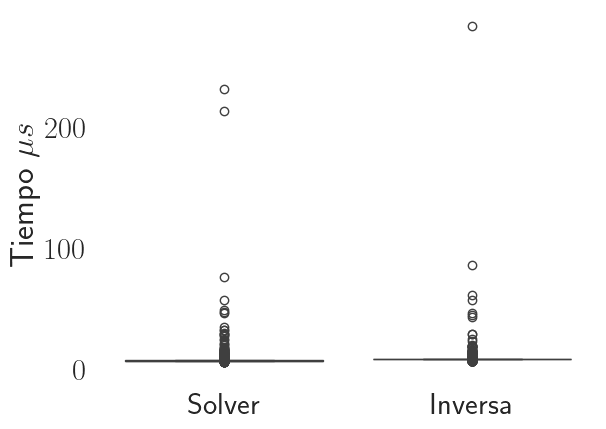
\includegraphics[width=0.5\textwidth]{../img/solver_inversa_gamma}
    \caption{Comparación de tiempos de cómputo entre Solver e Inversa}
    \label{fig:time_comparison}
\end{figure}

Los resultados se muestran en la Tabla~\ref{tab:solver_inversa_gamma}.

\begin{table}[H]
 \centering
\caption{Tiempo de ejecución de los métodos de solución}
\label{tab:solver_inversa_gamma}
\begin{tabular}{l|r|r}
 & Solver & Inversa \\ \hline
Media & 7.827 & 8.340 \\ \hline
Desviación estándar & 7.467 & 6.894 \\ \hline
Mínimo & 5.722 & 6.676 \\ \hline
Percentil 25 & 6.914 & 7.868 \\ \hline
Percentil 50 & 6.914 & 7.868 \\ \hline
Percentil 75 & 7.153 & 8.106 \\ \hline
Máximo & 230.789 & 283.241
\end{tabular}
\end{table}


De la Tabla~\ref{tab:solver_inversa_gamma}, se observa que el método de eliminación Gaussiana (Solver) es el más rápido en términos de tiempo de ejecución, en comparación con el método de inversa.
Este resultado es esperado, ya que el método de inversa requiere calcular la inversa de la matriz $I - \gamma P$, lo cual es computacionalmente costoso.

Por otro lado, se recomienda tener en cuenta este resultado al momento de seleccionar el método de solución a utilizar, ya que el tiempo de cómputo puede ser un factor importante en la elección del método.
Si bien el caso en particular no presenta diferencias significativas, en problemas más grandes, la diferencia en tiempo de cómputo puede ser considerable.

\line(1,0){\textwidth}


    \indent\underline{\textbf{Ejercicio 8}}\\
Demostrar que, dada una política estocástica $\pi (a \mid s)$, la función de valor de estado puede escribirse como

\[
    v_{\pi}(s) = \sum_{a \in \mathcal{A}} \pi(a \mid s) q_{\pi}(s, a)
\]

\indent\underline{\textbf{Solución}}\\

\line(1,0){\textwidth}


    \indent\underline{\textbf{Ejercicio 9}}\\
Demostrar que, dada una política estocástica $\pi (a \mid s)$, la función de valor de estado puede escribirse como

\[
    q_{\pi}(s,a) = \sum_{s',r} p(s', r \mid s, a) [r + \gamma v_{\pi}(s')]
\]

\indent\underline{\textbf{Solución}}\\
Sea,\\
$\pi(a \mid s)$: Política estocástica, es una función que asigna a cada estado $s$ una distribución de probabilidad sobre el conjunto de acciones $a$, es decir, $\pi(a \mid s) = P[A_t = a | S_t = s]$.\\
$q_{\pi}(s, a)$: Función de valor de acción bajo una política $\pi$, es el valor esperado del retorno a partir del estado $s$ y la acción $a$.\\
$p(s', r \mid s, a)$: Función de transición conjunta de estado y recompensas, es la probabilidad de que se obtenga el estado $s'$ y la recompensa $r$ al tomar la acción $a$ en el estado $s$.\\
$v_{\pi}(s)$: Valor de estado bajo la política $\pi$, es el valor esperado del retorno a partir del estado $s$.

La función de valor esperado de acción $q_{\pi}(s, a)$, se puede expresar como,
\[
    q_{\pi} (s,a) = E_{\pi}[R_t | S_t = s, A_t = a]
\]

Es decir, $q_{\pi}(s, a)$ es la suma de la recompensa inmediata $r$ y el valor esperado del retorno a partir del estado $s'$.
Al tomar la acción $a$ en el estado $s$ se obtiene la recompensa inmediata $r$ y se transiciona al estado $s'$.
Si se tiene en cuenta las recompensas futuras y todas las posibles transiciones y recompensas, la función de valor de acción se puede expresar como,

\[
    q_{\pi}(s,a) = \sum_{s',r} p(s', r \mid s, a) E[R_t \mid S_t = s', A_t]
\]

Las recompensas futuras se puede dividir en dos partes, que incluyen la recompensa inmediata $r$ y el valor esperado del retorno a partir del estado $s'$, ponderado por el factor de descuento $\gamma$,

\[
    E[R_t \mid S_t = s', A_t] = r + \gamma v_{\pi}(s')
\]

Al remplazar la expresión anterior en la función de valor de acción, se obtiene,

\[
    q_{\pi}(s,a) = \sum_{s',r} p(s', r \mid s, a) [r + \gamma v_{\pi}(s')]
\]

Entonces, el valor esperado total es igual al valor esperado de las recompensas inmediatas y futuras ponderadas por el factor de descuento $\gamma$~\cite{Sutton2018}.

\line(1,0){\textwidth}


    \indent\underline{\textbf{Ejercicio 10}}\\
Demostrar que la función de valor de estado óptima es

\[
    v_{\ast}(s) = \max_{a} q_{\ast}(s, a) = \max_{a} \sum_{s',r} p(s', r \mid s, a) [r + \gamma v_{\ast}(s')]
\]

\indent\underline{\textbf{Solución}}\\

\line(1,0){\textwidth}


    \indent\underline{\textbf{Ejercicio 11}}\\
\lipsum[4]\\

\indent\underline{\textbf{Solución}}\\

\line(1,0){\textwidth}


    \indent\underline{\textbf{Ejercicio 12}}\\
Demostrar que la función de valor estado-acción óptima es:

\[
    q_{\ast}(s,a) = \sum_{s',r} p(s',r \mid s,a) \left[ r + \gamma \max_{a'} q_{\ast}(s',a') \right]
\]

\indent\underline{\textbf{Solución}}\\
Sea,\\
$q_{\ast}(s,a)$: Función de valor de acción óptima, es el valor esperado del retorno a partir del estado $s$ y la acción $a$ bajo una política óptima.\\
$p(s',r \mid s,a)$: Función de transición conjunta de estado y recompensas, es la probabilidad de que se obtenga el estado $s'$ y la recompensa $r$ al tomar la acción $a$ en el estado $s$.\\
$v_{\ast}(s')$: Valor de estado óptimo, es el valor esperado del retorno a partir del estado $s'$ bajo una política óptima.

La función de valor de estado acción óptima $q_{\ast}(s,a)$, se puede expresar como,

\[
    q_{\ast}(s,a) = E[R_t | S_t = s, A_t = a]
\]

Es decir, $q_{\ast}(s,a)$ es la suma de la recompensa inmediata $r$ y el valor esperado del retorno a partir del estado $s'$~\cite{Sutton2018}.
El valor óptimo de la función de valor de acción se puede expresar como,

\[
    q_{\ast}(s,a) = \sum_{s',r} p(s',r \mid s,a) E[R_t | S_t = s', A_t = a]
\]

Donde,

\[
    E[R_t | S_t = s', A_t = a] = r + \gamma v_{\ast}(s')
    v_{\ast}(s') = \max_{a'} q_{\ast}(s',a')
\]

Al sustituir en la función de valor de acción óptima, se obtiene,

\[
    q_{\ast}(s,a) = \sum_{s',r} p(s',r \mid s,a) \left[ r + \gamma \max_{a'} q_{\ast}(s',a') \right]
\]

\line(1,0){\textwidth}


    \bibliography{references}

\end{document}
